%!TEX root = ../Demo.tex
\chapter{绪论}
\section{研究背景及意义}
随着智能设备的普及,设备的安全问题也受到了更多的关注。可信执行环境(Trusted Execution Environment,TEE)是由Global Platform所提供的定义,通过在中央处理设备中建立一套安全性范围,以确保其内的应用和数据信息在秘密性和完全性上得到保障。可信执行环境的原理是,把操作系统的硬件和软件资源区分为两种运行环境——即可信执行环境(TEE)和普通执行环境(REE)。这两种环境都是相互安全隔离并且共存的运算环境,都具有各自单独的内存数据通路和计算所需要的空间。TEE为REE提供了部分安全服务,如指纹认证、支付、数字认证等,而且有它自己的执行环境,安全等级也较普通环境中的操作系统高。同时,普通运行环境的应用程序也无法访问TEE,原因就是在TEE里面,各个应用的程序也是彼此独立的,所以不能因为无权限而互访。TEE也提供了安全性与成本上的均衡,可以满足大部分应用的安全性要求。与多方安全计算和联邦学习这些纯软件方面的解决方案比较,TEE可以支撑更多的算子和复杂运算,还可以进行关联运算、协同查询、联合建模和预测等各种运算,业务表达性更强。同时,TEE支持多层次、高度复杂的算法逻辑实现,计算效率极高。

TrustZone是ARM处理器系列提出的一种TEE技术,该安全扩展提供了在一个隔离的执行环境中保护安全敏感数据的功能。TrustZone已被广泛地应用于各种商业产品和学术项目\cite{zhang2016case,azab2014hypervision,zhou2014armlock,jang2015secret},以实现安全处理。受保护的环境被称为安全世界,而普通的操作系统运行环境被称为普通世界或不安全的世界。原理上,一个处理器上可以运行两个独立的操作系统,一个是运行在普通执行环境上的Linux,另外一个就是运行在可信执行环境之上的小内核(kernel),它结构简单,代码少,攻击面小,从而安全性得到了提高。由于ARM架构确保了许多硬件系统资源都是双份的,因此每个世界中的虚拟中心可以独享自身的那份资源,大大简化了设计。

与别的资源不同的是,cache是安全世界与普通世界共用的。为了区分,启用TrustZone的处理器的高速缓存行另外扩展了一个标志(NS)位,以指示当前的高速缓存行的作用域。安全世界对于cache使用的权限要远远大于普通世界。对于普通世界,处理器会无视这个NS标志位,对于安全世界,处理器需要按照对应的NS位,以安全世界或者普通世界的身份进行地址转换。尽管安全世界的缓存行不能被普通世界访问,但在争夺缓存行的时候,两个世界是平等的。当处理器在一个世界运行时,如果目标缓存组已满,它可以驱逐另一个世界使用的缓存行。这种缓存设计的存在,使得两个环境切换期间,不需要重新刷新高速缓存,以此可以提高系统性能。同时,两个世界对这些高速缓存的访问模式是类似且不受保护的,这使TrustZone很容易受到高速缓存侧信道攻击,具体来说,攻击者虽然无法直接获得TrustZone内程序执行的过程,但是通过间接获取缓存的数据变化情况,获得TrustZone中的安全应用的数据信息,从而获取一些秘密值。
\section{国内外研究现状}
传统的密码分析侧重于算法层面,利用算法在执行上的漏洞进行密码破解。而侧信道攻击利用了加密算法在执行时,软件或硬件泄露的信息,进行侧面信息提取,从而进行重要信息的破解。

侧信道攻击在计算机安全领域有较广泛的应用\cite{kocher1999differential,kocher1996timing},同时也有许多防御手段\cite{王崇2021缓存侧信道防御研究综述}。随着对缓存的大量研究,缓存侧信道攻击在学术界也吸引了众多学者的视线。使用侧信道信息作为攻击加密方案的手段的概念首次出现在\cite{kocher1996timing}的一篇开创性论文中。在\cite{kocher1996timing}中,Kocher利用计算时间的差异来破解RSA和基于离散对数的加密算法的实现。除了时间,其他物理属性,如电磁辐射\cite{genkin2016ecdsa}、功耗\cite{kocher1999differential}或声学噪音\cite{genkin2014rsa}也被研究为可行的侧信道来源。Bernstein\cite{bernstein2005cache}是第一个表明由数据缓存,会存在时间依赖性的学者,这使得AES\cite{bernstein2005cache}的T table实现能够被攻击并恢复出密钥。基于缓存的侧信道攻击有三个类别:时间驱动\cite{bernstein2005cache},跟踪驱动\cite{aciiccmez2006trace}和访问驱动\cite{percival2005cache}。它们之间的区别在于攻击者的能力,其中时间驱动性攻击限制最少。

Osvik等人\cite{osvik2006cache}提出了两种技术供攻击者确定受害者访问的缓存集,即 evict+time 和 prime + probe。在evict + time中,攻击者修改一个已知的缓存集,并观察受害者的加密操作的执行时间的变化。在prime + probe中,攻击者在执行加密操作之前用已知的状态填充缓存,并在执行完加密操作后,观察这些缓存状态的变化。 Gullasch等\cite{gullasch2011cache}确定了另一个由系统内存删除而得来的缓存侧信道攻击。攻击者在启用KSM的情况下,冲刷恶意进程和受害者进程之间共享的内存,如加密库。在受害者执行加密算法后,攻击者测量将内存载入寄存器的时间,以确定该内存是否被受害者进程访问过。后来Yarom等人在\cite{yarom2014flush+}中将这种缓存攻击方法命名为flush+reload。国内学者也对该缓存侧信道攻击方法进行了扩展,研究了差分flush+reload的攻击方法\cite{袁稚炜2019基于差分}。随着人们对云计算的兴趣越来越大,另一个研究方向\cite{ristenpart2009hey,zhang2012cross}专注于从虚拟机而不是本地机器的进程中恢复秘密。

目前的研究大多集中在对英特尔x86架构处理器的侧信道调查上,但很少涉及ARM平台。Weiss 等人\cite{weiss2012cache}首次在ARM处理器中测试了Bernstein攻击。除了Bernstein的定时攻击,在\cite{lipp2016armageddon}中使用了evict+time来攻击AES的T表实现。在\cite{zhang2016return}中还使用了内存复制来发起flush+reload攻击,以跟踪共享库的执行路径。Lipp等人\cite{lipp2016armageddon}针对ARM处理器,利用Java来实现缓存攻击以恢复加密密钥,同时,他们能够在TrustZone中监视缓存活动。与\cite{lipp2016armageddon,zhang2016return}相比,在此篇文章中,我们的研究目标是不同的。由于TrustZone的内存分离保护,普通世界和安全世界在执行时的内存是分离的,而evict + reload\cite{lipp2016armageddon}或flush + reload\cite{zhang2016return}都需要基于内存共享的前提,在本课题中,无法使用上述两种方法。故在本文的研究中,我们可以使用prime+probe方法对缓存进行信息提取并攻击加密密钥,在\cite{lipp2016armageddon}中作者简要地讨论了prime+probe的可行性。在\cite{zhang2016truspy}中,Zhang等人针对ARM TrustZone环境,提出了第一个基于时间的侧信道攻击。除了缓存定时侧信道,最近的一项研究证明了一个新的缓存侧信道攻击,基于缓存不连贯性的意外缓存命中\cite{guanciale2016cache},该攻击可以从Cortex-A7处理器的安全世界中恢复秘密值。

基于\cite{zhang2016truspy}中的对缓存的时间侧信道攻击,我们同样针对ARM TrustZone环境,进行缓存的攻击实现,同时尽可能提升攻击效率和准确度。在我们的攻击方案中,利用了操作系统sudo权限,触发安全世界中的加密执行,并且探测共享的缓存在加密前后的数据变化。本文所利用的缓存时间侧信道攻击是基于ARM TrustZone的特性进行设计的。TrustZone在缓存中添加一个额外的标志位来标识当前的缓存行是安全世界还是普通世界是使用的,而不采用缓存分离机制。任意一个世界在执行程序时,如果数据地址对应的缓存组已经被占满,就会遵循一定策略实行缓存驱逐,这时候缓存的数据状态就会发生改变,攻击者端使用一定的探测方法就能知道受害者使用的具体数据,为本文研究的缓存攻击提供了一定的先决条件。
\section{研究内容和组织框架}
\subsection{研究内容}
我们在Cortex A-53处理器的Raspberry Pi 3B开发板上实现了TrustZone缓存侧信道攻击,以一个基于T-表的AES实现为例,展示了TrustZone的侧信道信息泄漏。来自正常世界的攻击可以观察多次加密过程中缓存的数据变化,并且恢复完整的AES128的16位密钥,本文工作可以归纳为以下三点:
\begin{enumerate}[label=(\arabic*)]
	\item 基于TrustZone中普通世界和安全世界之间的缓存设计架构,成功识别并利用了缓存的侧信道信息,该架构允许两个世界共享相同的缓存来提高系统性能。
	\item Prime+Probe是Intel架构上采用的较广泛的缓存攻击方法,本文详细介绍了该技术在ARM处理器上的采用,其中有许多难点,例如缓存替换策略的随机性、无法中断加密过程、缺少rdtsc指令直接获取cache miss次数以及CA和TA交互过程设计。
	\item 在得到缓存数据信息变化后,利用不同位置(如缓存、内存)的数据加载在时间上的差异性,结合缓存侧信道可行性分析,得到加密过程中的加密密钥。 
\end{enumerate}
\subsection{组织框架}
本文的结构安排如下:

第一章: 阐述该课题的科研背景、重要性以及国内状况,并提出本文的科研内容与组织架构。

第二章:介绍本课题涉及的关键技术领域,ARM TrustZone的运行机制、内存结构在程序运行时对地址的加载以及现有的缓存侧信道攻击方法。

第三章:介绍本课题利用的攻击模型及合理假设。

第四章:阐述本课题攻击的对象,即OpenSSL的AES128加密过程,以及如何利用缓存配置和加密密文攻击密钥的原理。

第五章:具体分析并阐述本课题的实验方法。

第六章:对上述实验方法进行具体实验,以验证方法的可行性和算法的效果,并介绍应对缓存攻击的可能的方法。

第七章:对本课题所采取的攻击方法加以总结,并同时给出了对今后工作方向的展望。
\chapter{关键技术}
\section{ARM TrustZone}
ARM TrustZone是基于硬件的安全功能,它通过对原有硬件结构进行了调整,并在处理器层次引入了两种不同权限的工作域——安全世界和普通世界,任何时刻处理器都只在其中的一种环境内工作。而且由于这二种世界之间全部是以硬件分隔的,并且有不同的权限,在普通世界中运作的软件访问安全世界中的信息或资源是被严格控制的,反过来在安全世界中运行的应用能够正常访问普通世界中的数据。

一旦处理器的操作状态被划定,普通世界状态下的Linux即使以root身份进行操作,也不能访问安全世界状态下的任何资源,包括设备、内存数据、获取缓存数据等。无论外部环境是否安全,安全世界内的执行都是安全的。这是因为当CPU访问安全设备或安全存储器地址空间时,芯片级安全扩展组件检查CPU发送的访问请求的读/写安全状态信号(非安全位,NS位)是否等于0或1,以确定CPU发送的当前资源访问请求是安全请求还是普通请求。当普通世界的CPU发送系统总线访问指令时,访问请求的读/写安全状态信号位被强制为1,表明当前CPU的访问请求是普通世界的操作请求。当普通请求试图访问一个安全世界的资源时,它将被安全扩展组件视为不安全的请求,对受保护资源的访问将被禁止。

两个世界间的硬件隔离以及不同的权限等功能,保障了正常应用程序代码与数据的有效机制:普通世界(Normal  World)通常用于运行操作系统(如安卓、iOS等),提供普通运行环境(Rich Execution Environment,REE);安全世界(Secure World)总是使用安全环境或者安全内核(TEE-kernel),建立可信的执行环境(Trusted Execution Environment,TEE),可以存储和访问敏感数据。这样一来,即使正常情况下的操作系统被损坏(如iOS被黑客攻击或Android系统被获得ROOT权限),黑客仍然无法访问存储在TEE中的敏感数据与重要信息。

图\ref{001}描述了Cortex-A上采用的TrustZone架构。普通世界(或非安全世界)与安全世界之间,存在着一种监视模式(Monitor  mode)的处理器模式,该模式负责在两个世界过渡时保留处理器状态。普通世界中可以通过调用安全监视器(SMC)的特权指令进入监视模式;此时执行在监视模式的代码首先保存在普通世界中的CPU上下文,将CPU中的NS位置为零,然后进入安全世界的特权模式;安全世界的操作系统唤醒安全世界中的应用处理完相应的资源访问请求后,也会发送SMC指令,再次回到监视模式;运行在监视模式的代码同样保存安全状态下的CPU上下文,再重新回到普通世界特权模式。

\begin{figure}[H]
	\centering
	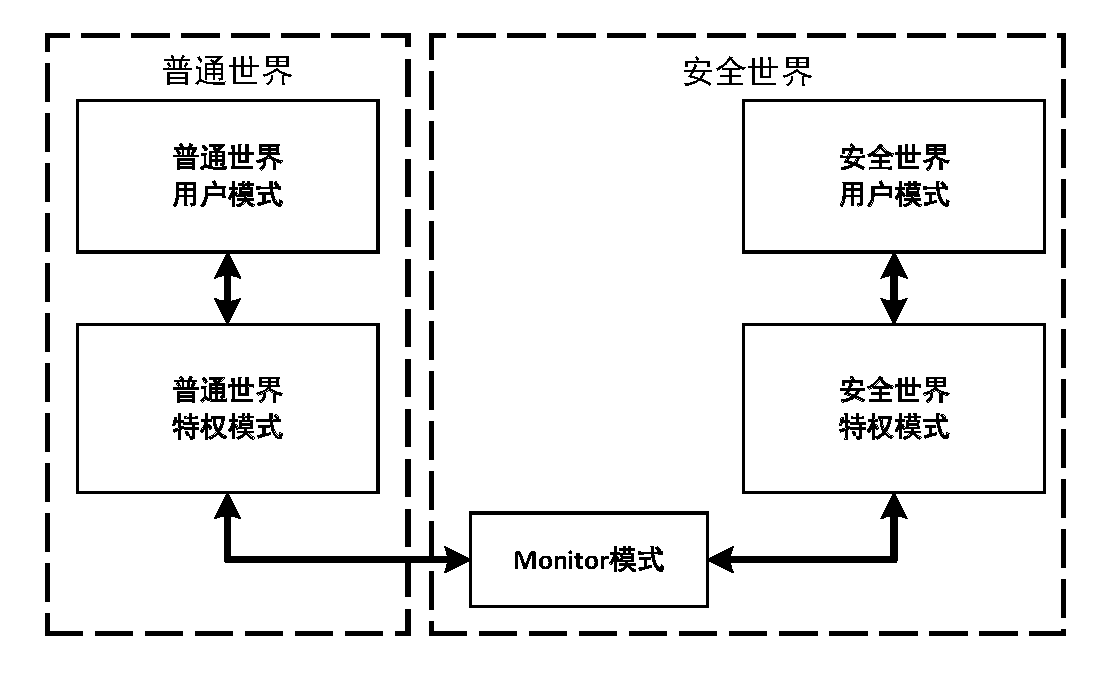
\includegraphics[width=0.7\textwidth]{001.png}
	\caption{Cortex-A上的TrustZone架构}
	\label{001}
\end{figure}

\section{处理器内存层次架构}
本文的攻击环境是基于ARMv7l 架构的Cortex-A53处理器搭建的,故在本节重点介绍Cortex-A53处理器的内存层次架构。
\subsection{内存与Cache的映射关系}
现代计算机系统中,程序在虚拟地址空间中运行,当处理器需要在内存中获取一个值时,它将虚拟地址传递给内存管理单元(MMU),MMU首先从旁路快表缓冲(TLB)中检索虚拟地址到物理地址的转换。若没有找到对应项,MMU就解析页表,并将解析得到的物理地址放入TLB中,以提高下一次同一地址的查询速度。一旦获得物理地址,CPU就通过访问系统内存来获得该地址的值。

现代处理器通常有多级缓存结构,以实现更快的内存访问。缓存的层次越高,速度越快,并且越靠近核心处理器。在上述CPU通过访问内存来获取数据前,缓存控制器会先检查要获得的数据是否在缓存中,若在缓存中,则CPU可以直接从缓存中获取数据,速度较快,这称为一次缓存命中(cache hit)。若不在缓存中,则需要从内存中把数据先加载到缓存中,再加载至CPU寄存器中,速度较慢,这个过程称为缓存未命中(cache miss)。与物理内存相比,缓存的尺寸通常较小,其中的数据只占内存的一小部分。缓存命中率越高,数据载入时间就越少,整体运行速度就越快。Cortex-A53拥有4个核,可以查看核的Online或Offline状态,整体是两级缓存配置,每个核都有可配置的16$-$64KB的L1指令缓存(L1i Cache),16$-$64KB的L1数据缓存(L1d Cache),并且这1$-$4个处理器之间有共享的128KB$-$2MB的L2缓存。

缓存中内存分配的基本单位为缓存项,一个缓存项由标签、缓存行和若干标志位组成,每个缓存行一般为64字节。多个路的缓存项组成一个缓存组,多个组再组成整个缓存。高速缓存通常采用N路组相联映射。在本文所研究的环境中,每个缓存行大小均为64字节,L1数据缓存则由128组的4路缓存项构成,即大小为32KB。第二级缓存由16路组相联构成,共有512组,每个缓存行大小也为64KB。由于TrustZone的加入,每个缓存行都被扩展了NS位,它指定了该缓存行的状态,这个设计的目的是使用NS位来区分当前这个缓存行是安全世界的还是普通世界的数据,世界切换时则不需要刷新缓存,以此提高运行效率。
\begin{figure}[H]
	\centering
	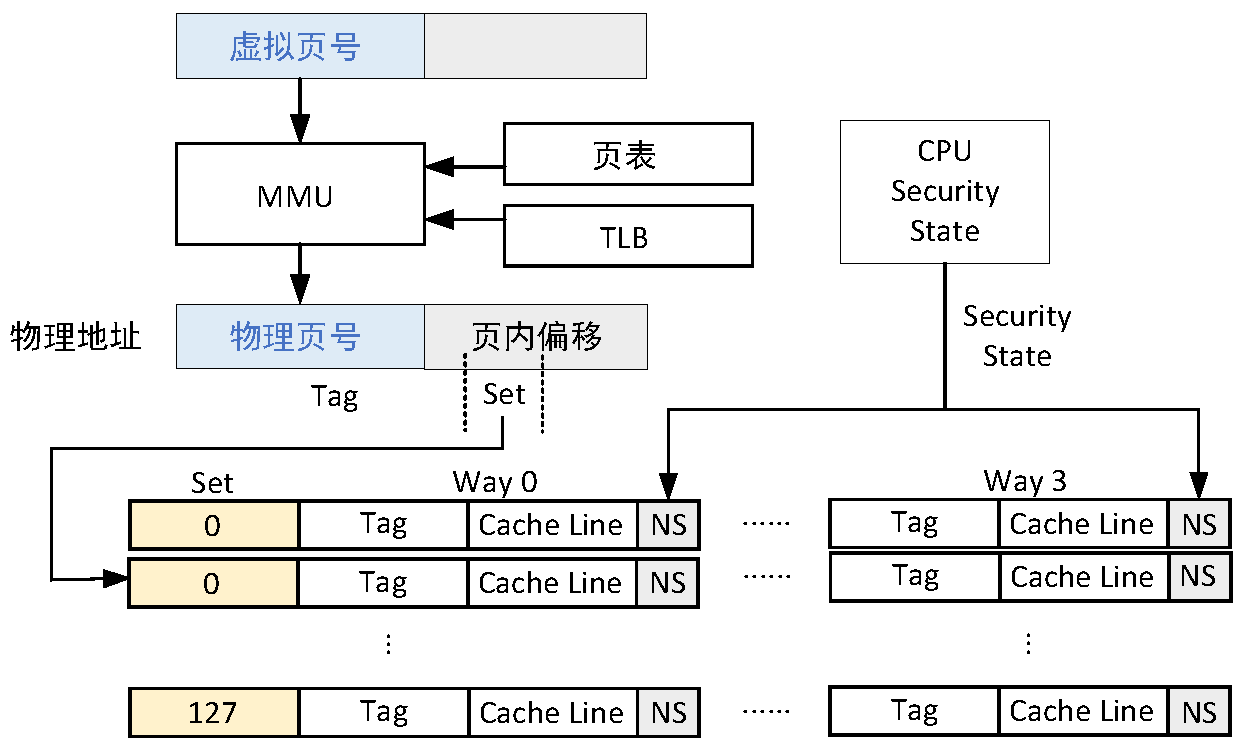
\includegraphics[width=0.8\textwidth]{002.png}
	\caption{ L1D Cache抽象图以及内存层级结构}
	\label{002}
\end{figure}


由于缓存容量相对内存来说非常小,仅能存储内存中一部分数据,故需要构建物理地址到缓存的映射,以确认目标缓存中的数据是否为目标物理地址的数据。由于我们的主要攻击对象为数据缓存,图\ref{002}为L1D Cache的抽象图以及整体的内存层级结构。对于一个32位的地址来说,第0-5比特位为缓存行内的偏移,第6-12这7个比特位为缓存组的映射,匹配相应的缓存组后,用13-31比特位匹配这个缓存组中的4个缓存项的标签,若有能匹配上的,这个缓存行的内容即目标内存的内容,可以直接加载进寄存器进行数据操作。若没有能够匹配上的标签,需要去L2或者内存中查询数据,速度相对慢很多。


\subsection{Cache的驱逐与替换}

上述提到,缓存的大小要远远小于内存大小,当发现目标数据此时还没有被加载到L1数据缓存中,缓存控制器会去L2缓存中寻找目标数据。若此时仍未找到,处理器会从RAM中取出数据,并把数据放到缓存中,此时若物理地址对应的缓存组已满,必定会驱逐之前已经填到该缓存组中的某个缓存行。这就是缓存驱逐。同时,不管是安全世界还是普通世界的缓存行,在任意一个世界执行时都有可能被驱逐,以便为新的数据腾出空间。换句话说,安全缓存行的填充有可能会驱逐普通缓存行,反之亦然。这种设计是对TrustZone中受保护的执行进行侧信道攻击的关键。

在进行缓存替换时,CPU对32位物理地址进行拆分,先计算这个地址的缓存组映射,然后在组内使用缓存替换算法,从这个缓存组的4个缓存项中挑出一个,把原有的数据驱逐,放入更新的数据,其中,需要更新64字节的缓存行部分,19比特的标签部分,以及NS位等。

在现代的ARM架构中,内存系统通常有多个层次,缓存是最高级别的,且缓存通常分为多个级别。许多ARM处理器中的高速缓存既不是包容性的,也不是排他性的,也就是说最高级别缓存中的缓存行不一定会存在低级缓存中。ARM处理器的缓存控制器的替换策略是随机替换策略。缓存替换策略指的是,当出现高速缓存竞争时,处理器从每组的n个(本文中是4个)缓存行中如何选择一个驱逐并进行新的缓存替换。随机替换策略给实验新增一个难点,即如何确保当前的数据加载进缓存时,之前的数据没有被驱逐,解决方法将会在第五章攻击方案中介绍。

虽然从内存加载数据和从缓存加载数据的时间差比较明显,但由于缺乏缓存包容性,若在攻击过程中以低级别的缓存作为目标会使分析过程变得比较困难。如果将高级别的缓存作为侧信道攻击的对象,数据加载的时间区别最明显。同时,只要是处理器访问的内存数据,一定会被先放到L1数据缓存中。故在实验中,我们主要以L1数据缓存作为观测的对象,以此来捕捉高速缓存争夺中的信息泄露。

Linux操作系统中,所有程序在运行时采用的都是逻辑地址,而逻辑地址会被MMU变换为物理地址,再用这个物理地址向RAM发出内存读写请求,每个内存块的大小为4KB。故物理地址的最低12位为页内偏移。因为L1D cache一共有128个缓存组,在将逻辑地址转化为物理地址时,页内偏移的0-11位是不会改变的,只有第12位为0或1,也是攻击者无法完全控制的。故在求缓存组映射时,逻辑地址的第12位转化成物理地址后,决定会映射到前64还是后64个缓存组,加上不变的6-11位就可以完全确定映射到的缓存组号。在实验中,由于第12位转化成物理地址后是无法获取的,需要对该位为0或1的情况分别进行确定。而逻辑地址可以直接通过可执行连接文件.elf或动态链接库.so通过以下命令(示例中是获得4张Te表的偏移)查看。

\begin{lstlisting}[language=shell]
	 nm target.elf | grep Te[0-3]
\end{lstlisting}




\section{缓存侧信道攻击}
\subsection{现有的cache攻击手段}
缓存侧信道攻击的本质是通过缓存创建一个通道,通过这个通道可以获得某些隐藏的信息,以检测程序是否访问了某个特定内存地址的数据。例如,攻击者能够在内存(缓存未命中)与缓存访问数据(缓存命中)的时间差值中了解缓存上的信息或数据的变动。下面是几种缓存攻击基本手段。

\textbf{Flush+Reload:}

Intel处理器提供了clflush执行,针对于一个地址进行操作,可以将这个地址的数据从缓存中驱逐。Flush+Reload方法基于共享内存实现,是一种跨内核的缓存探测方法。第一步,攻击者使用clflush指令把目标地址从缓存中驱逐,然后在下一阶段,受害者程序触发执行。最后一步,攻击者访问目标地址的数据,并记录访问时间。若访问过的内存块已经在缓存中而不需要reload,时间会相对短一些,因为缓存命中的加载时间较短。根据记录的时间结合一定阈值,可以判断受害者程序是否使用过这部分数据。Flush-Reload具体步骤说明:

\begin{itemize}
	\item Step 1. Flush: 使用clflush指令把目标地址从缓存中驱逐
	\item Step 2. Trigger:触发目标(受害者)程序执行
	\item Step 3. Reload:重新访问内存中的那个数据,测量并记录时间
\end{itemize}


\textbf{Flush+Flush:}

该攻击方法同样是基于clflush指令执行时间的长短来实施攻击的。如果数据未在Cache中,clflush指令执行时间会比较短,相反,有数据在cache中则执行时间会比较长。与其它Cache攻击不同,Flush+Flush侧信道攻击技术在整个攻击过程中是不需要对内存进行存取的,所以该攻击技术也较为隐秘。Flush+Flush具体步骤如下:

\begin{itemize}
	\item Step 1. 通过clflush指令驱逐目标地址在缓存中的数据
	\item Step 2. 触发受害者程序运行
	\item Step 3. 再次利用clflush指令驱逐共享缓存行,测量刷新时间;根据测量时间判断原始数据是否被缓存,如果时间超过一个阈值,则认为此时对应的缓存中是有数据的,那么攻击者被看作访问了该地址的数据。
\end{itemize}

\textbf{Evict+Time:}

Evict+Time具体步骤如下:

\begin{itemize}
	\item Step 1. 攻击者将目标地址的数据填入缓存
	\item Step 2. 触发受害者程序运行,并记录其运行时间,运行过程有可能使用到第一步中的缓存数据
	\item Step 3. 使用Evict方法驱逐Cache上的数据
	\item Step 4. 然后再运行一次该函数,并第二次记录执行时间,如果时间不一致且执行时间变长则说明程序运行时读取了第一步所说的Cache数据(Cache未命中)。
\end{itemize}

\textbf{Prime+Probe:}

该方法与上面三种不同的是,不需要共享内存的环境就可以进行攻击。Prime+Probe方法具体步骤如下:

\begin{itemize}
	\item Step 1. Prime: 攻击者用预先准备的内存数据填充目标的cache 组(set)
	\item Step 2. Trigger:触发受害者程序的执行,等待它将cache数据更新
	\item Step 3. Probe: 重新遍历Prime 阶段填充的数据,测量并记录各个cache组读取时间,利用时间差来判断当前的数据加载是从内存中还是从高速缓存中直接读取
\end{itemize}

上述四种缓存侧信道攻击方法中,由于指令clflush在JavaScript和非Intel CPU中无法使用,所以最后一种方法较前几种方法更加常用。但同时,Prime+Probe在攻击速度、攻击稳定性方面,不如Flush+Reload和Flush+Flush这两种方法。本文攻击环境是ARM,故将采用最后一种攻击方法,具体原因及原理将在下一步阐述。

\subsection{针对TrustZone的攻击方法}
上述的evict+time,flush+reload,flush+flush这三种cache攻击方法必须基于共享内存,由于TrustZone的内存分离保护,这三种方法都无法使用。故必须使用prime+probe这种方法,因为它不需要共享内存的前提,只需要知道目标数据的物理地址或虚拟地址,即可进行缓存组的映射。TrustZone中的缓存项虽然存在NS位来区分是安全世界还是普通世界使用的,但是缓存驱逐时是不考虑现有的NS位的,只要对应到目标缓存组,就会在缓存组里进行驱逐与替换。

Prime+Probe攻击中,需要先构造一个驱逐集。为了在攻击后半部分的probe步骤中获得关于受害者进程的秘密信息,攻击者必须在prime阶段准确地将特定地址的内存内容填充到目标缓存区域,这样它就会引起与受害者进程的缓存争用。为了构造驱逐集,攻击者需要找到同样会被映射到受害者进程使用的缓存组的内存地址。以一定次数执行这部分内存地址的数据遍历,这些数据就会被填充到目标缓存组。当受害者程序访问了同样映射到这个缓存组的数据时,原本构造的占用整个缓存组的4个缓存项将会有一个被驱逐到内存中,新的数据就会替换。再执行一遍prime过程遍历的数据,会有某项数据的访问时间明显与其它数据的访问时间不同,这就是从内存访问数据和直接从缓存中访问数据的巨大的时间差造成的。通过比较这个时间阈值,可以得知当前的数据是否在安全世界执行某个任务时用到这个缓存行,这样一来,本不应该被获得的秘密信息就可以通过这个时间被攻击者获取,从而进行一些更深入的探测和攻击。



\chapter{攻击模型及假设}
\begin{figure}[H]
	\centering
	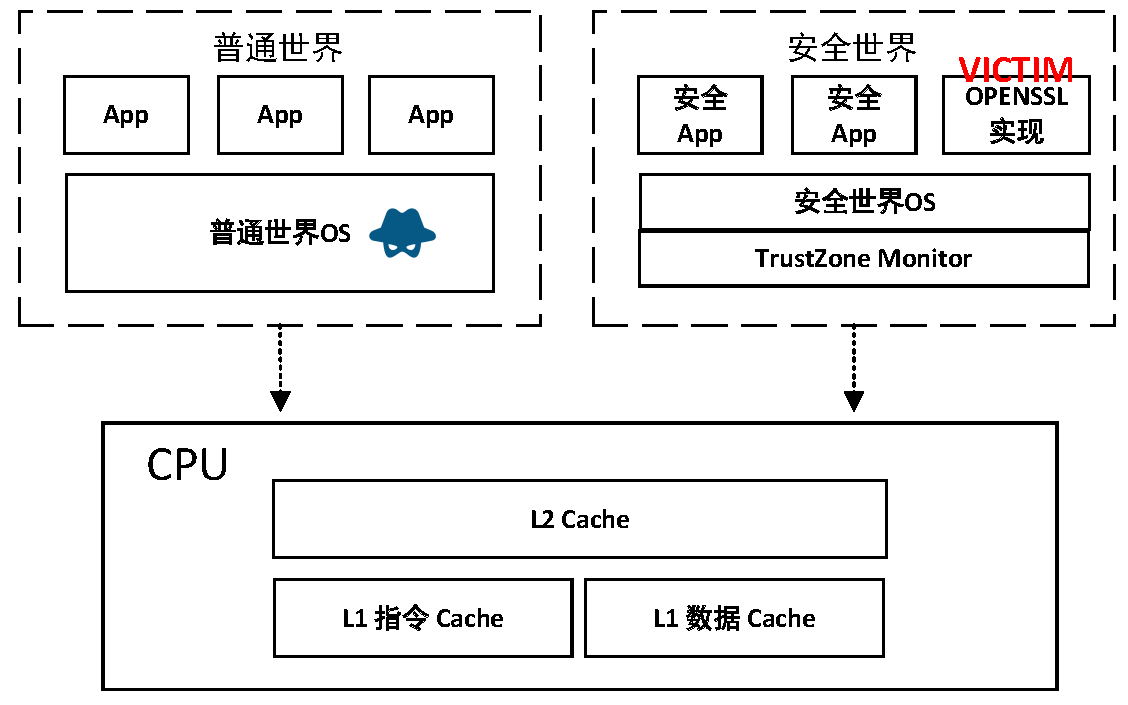
\includegraphics[width=0.9\textwidth]{003.png}
	\caption{TrustZone cache攻击模型}
	\label{003}
\end{figure}

本章介绍文章中涉及的攻击方案的模型及假设。

正如ARM TrustZone白皮书\cite{holdings2009arm}所说,TrustZone通常用来在高度隔离的执行环境中保护涉及安全数据的应用 ,例如加密操作。假设有一ARM架构的设备,其中普通世界内核为Linux系统,安全世界为TrustZone,攻击目标是获取安全世界运行的某个程序中涉及的秘密值,如AES加密过程中的16位密钥。同时假设加密库在安全世界中得到保护,并且没有受到在普通世界中运行的可能被损坏的操作系统的干扰,也就是说无法被普通世界进行直接攻击。

攻击模型如图\ref{003}所示。假设有一个openssl的aes加密过程在安全世界实现,并为普通世界的操作系统提供安全服务。普通世界的攻击者拥有操作系统的最高权限,即可以以sudo权限执行任意代码,这种假设在对硬件强制执行的可信环境发起攻击时是非常常见的。攻击目标就是安全世界的openssl的AES加密模块中的16位随机初始化的密钥。我们认为攻击者可以触发受害者进程中的加密,同时为受害者进程提供16位明文,经过加密后可以获得16位密文。同时,攻击者可以利用内核中的性能监测单元(PMU)模块随时获取执行过程的CPU周期数,观察从不同位置加载进寄存器的时间在CPU周期上的差异性。



\chapter{攻击对象}

\section{OpenSSL AES}
高级加密标准(Advanced Encryption Standard, AES),也被叫做Rijndael加密法,若按算法流程直接进行加解密操作,可能会有计算量大、耗时长等问题。为解决这些问题,我们通过用简单的查表操作代替一些复杂的过程来降低算法的时间复杂性,以此更好地优化算法。整个加密过程,可概括为字节替代(SubBytes)、行移位(ShiftRows)、列混合(MixColumns)和轮密钥加(AddRoundKey)。其中,本文专注于研究AES的128位加密算法,并且主要攻击最后一轮的16字节密钥。因为密钥计算过程是可逆的,我们可以通过最后一轮的密钥倒推出最初的16字节密钥。整体的AES加密过程如图\ref{004}所示。

\begin{figure}[H]
	\centering
	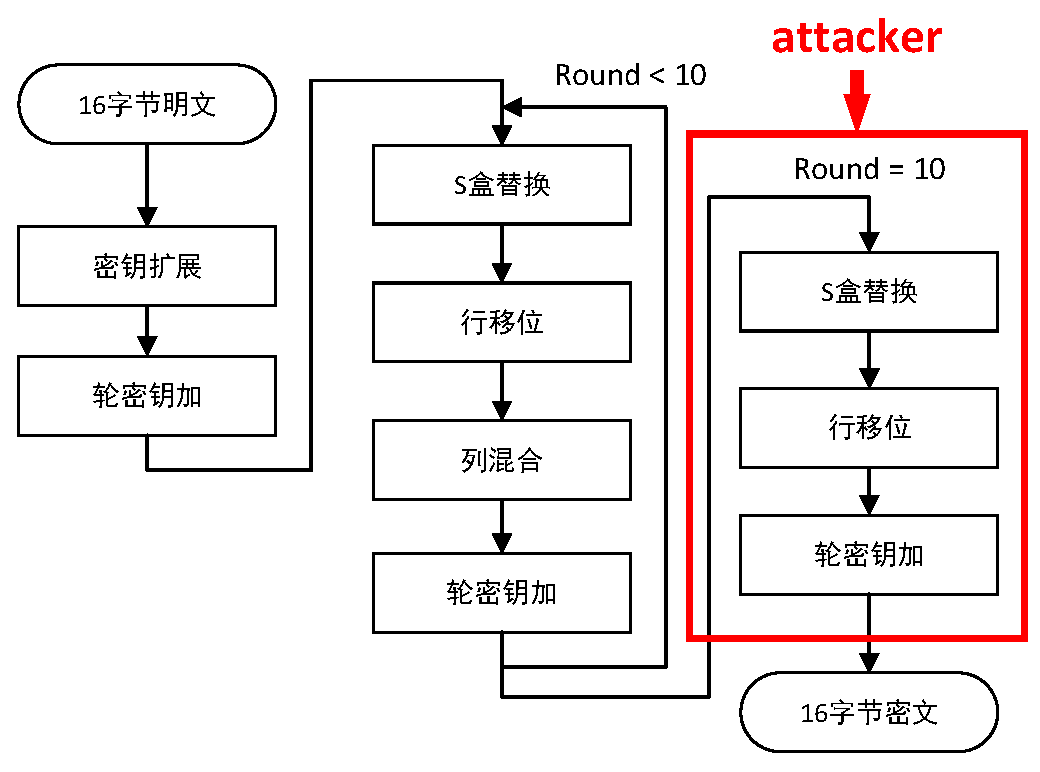
\includegraphics[width=0.8\textwidth]{004.png}
	\caption{AES加密过程}
	\label{004}
\end{figure}

下面对AES的T表概念进行解释。规定以下符号概念:

\begin{table}[H]
	\centering
	\caption{符号解释}
	\setlength{\tabcolsep}{16mm}{
	\begin{tabular}{cc}
		\hline \hline
		符号&解释\\
		\hline
	${p_{ij}}$ & 明文字节\\
	${p_{ij}^{'}}$ & 前一轮输入字节经一轮后生成的中间字节\\
		${k_{ij}}$ & 轮密钥\\
		${c_{ij}}$ & 密文字节\\
		$SBox\left[  \cdot  \right]$& S盒查询\\
		$\oplus$ & 异或\\
		$||$ & 连接符号\\
		${P_j}$ & ${p_{1,j}}||{p_{2,j}}||{p_{3,j}}||{p_{4,j}},0 \le j \le 3$\\
		${C_j}$ & ${c_{1,j}}||{c_{2,j}}||{c_{3,j}}||{c_{4,j}},0 \le j \le 3$\\
		${K_j}$ & ${k_{1,j}}||{k_{2,j}}||{k_{3,j}}||{k_{4,j}},0 \le j \le 3$\\
		$TBox\left[  \cdot  \right]$ & TBox\\
		$Te\left[  \cdot  \right]$ & Openssl中简化计算后的T表\\
		\hline \hline
	\end{tabular}}
	\label{table1}
\end{table}

我们将输入的16字节明文看作一个4*4的矩阵,矩阵的每一格代表一个字节,并且竖着的一列表示连续的4个字节。即一个明文输入可以看作${P_1}||{P_2}||{P_3}||{P_4}$,共16个字节。

\textbf{S盒替换:}

对于每一格输入${p_{ij}}$,把该字节的高4位看作行,后4位看作列,以行列为索引在S盒中找到替换后的字节, $p_{ij}^{'} = SBox\left[ {{p_{ij}}} \right]$。

\textbf{行移位:}

左循环移位操作,上一步输出的4*4状态矩阵中,第0行左移0字节,第1行左移1字节,以此类推,$p_{ij}^{'} = {p_{i,i + j}}$。

\textbf{列混合:}

通过矩阵相乘的方式实现,通过将行移位后的状态矩阵和固定的矩阵相乘,得到列混合后的新状态矩阵,过程如下式给出。

\begin{equation}
	\left[ \begin{array}{l}
		p_{0,0}^{'}\;p_{0,1}^{'}\;p_{0,2}^{'}\;p_{0,3}^{'}\\
		p_{1,0}^{'}\;p_{1,1}^{'}\;p_{1,2}^{'}\;p_{1,3}^{'}\\
		p_{2,0}^{'}\;p_{2,1}^{'}\;p_{2,2}^{'}\;p_{2,3}^{'}\\
		p_{3,0}^{'}\;p_{3,1}^{'}\;p_{3,2}^{'}\;p_{3,3}^{'}
	\end{array} \right] = \left[ \begin{array}{l}
		02\;03\;01\;01\\
		01\;02\;03\;01\\
		01\;01\;02\;03\\
		03\;01\;01\;02
	\end{array} \right]\left[ \begin{array}{l}
		p_{0,0}^{}\;p_{0,1}^{}\;p_{0,2}^{}\;p_{0,3}^{}\\
		p_{1,0}^{}\;p_{1,1}^{}\;p_{1,2}^{}\;p_{1,3}^{}\\
		p_{2,0}^{}\;p_{2,1}^{}\;p_{2,2}^{}\;p_{2,3}^{}\\
		p_{3,0}^{}\;p_{3,1}^{}\;p_{3,2}^{}\;p_{3,3}^{}
	\end{array} \right]
\end{equation}

状态矩阵中每一项的列混合结果可以按如下表示,元素下标的加法运算若超出3则按模3计算:

\begin{equation}
p_{ij}^{'} = \left[ {02\;03\;01\;01} \right]\left[ {{p_{i,j}}\;{p_{i + 1,j}}\;{p_{i + 2,j}}\;{p_{i + 3,j}}} \right]
\end{equation}

其中,所有矩阵元素的乘法和加法都是定义在基于GF(256)的二元运算,而不是一般含义上的乘法和加法。矩阵元素的加法可以看作简单的异或操作。将列混合看作列上的操作后,可以得到如下的式子:

\begin{equation}
\begin{array}{l}
	P_j^{'} = p_{0,j}^{'}||p_{1,j}^{'}||p_{2,j}^{'}||p_{3,j}^{'}\\
	= (2{p_{0,j}} \oplus 3{p_{1,j}} \oplus {p_{2,j}} \oplus {p_{3,j}})||\\
	\quad (2{p_{1,j}} \oplus 3{p_{2,j}} \oplus {p_{3,j}} \oplus {p_{0,j}})||\\
	\quad (2{p_{2,j}} \oplus 3{p_{3,j}} \oplus {p_{0,j}} \oplus {p_{1,j}})||\\
	\quad (2{p_{3,j}} \oplus 3{p_{0,j}} \oplus {p_{1,j}} \oplus {p_{2,j}})
\end{array}
\end{equation}

将其中的异或和连接符号进行顺序调换并不影响计算结果,故顺序调换后,可以将计算过程简化成4个TBox的查表替换行为:

\begin{equation}
\begin{array}{l}
	TBo{x_0}[x] = 2x||x||x||3x\\
	TBo{x_1}[x] = 3x||2x||x||x\\
	TBo{x_2}[x] = x||3x||2x||x\\
	TBo{x_3}[x] = x||x||3x||2x
\end{array}
\end{equation}

此时列混合的步骤可以由如下表示:

\begin{equation}
P_j^{'} = TBo{x_0}\left[ {{p_{0,j}}} \right] \oplus TBo{x_1}\left[ {{p_{1,j}}} \right] \oplus TBo{x_2}\left[ {{p_{2,j}}} \right] \oplus TBo{x_3}[{p_{3,j}}]
\end{equation}

其中,$0 \le j \le 3$,故列混合操作可以看作对TBox的快速查询操作,每一列的变换通过原列中的4个字节,取表中拼接而成,得到4个字节,作为新一列的输出。其中每个TBox有256项,每一项为4字节。

\textbf{轮密钥加:}

将上述结果的每一项${p_{ij}}$与对应密钥进行异或操作,得到这一轮的输出。

以上为AES加密的四个步骤,而OpenSSL中,上述的四个步骤被整合为新的查找表$T{e_i}\left[  \cdot  \right]$,其中$0 \le i \le 3$:

\begin{equation}
T{e_i}\left[ x \right] = TBo{x_i}\left[ {SBox\left[ x \right]} \right]
\end{equation}

也就是说,前9轮的输出结果都可以看作是一次表的查询操作,有利于计算效率的提高。每一轮的输出可以看作如下表达式:

\begin{equation}
	P_j^{'} = T{e_0}\left[ {{p_{0,j}}} \right] \oplus T{e_1}\left[ {{p_{1,j + 1}}} \right] \oplus T{e_2}\left[ {{p_{2,j + 2}}} \right] \oplus T{e_3}\left[ {{p_{3,j + 3}}} \right] \oplus {K_j}
\end{equation}

对于最后一轮加密,因为少了列混合的步骤,故最后一轮可以用如下式子表示:

\begin{equation}
	p_{i,j}^{'} = SBox\left[ {{p_{i,i + j}}} \right] \oplus {k_{i,j}}
\end{equation}

因为Te表就是由S盒经过一定变换得到的,故最后一轮的输出也可以由Te表项得到。首先,最后一轮的输出密文可以由如下式子表示:

\begin{equation}
	{c_{ij}} = SBox\left[ {{p_{i,i + j}}} \right] \oplus {k_{ij}}
\end{equation}

其中,S盒的内容可以通过Te表间接得到,以$T{e_0}$为例:

\begin{equation}
	\begin{array}{l}
		T{e_0}\left[ x \right] = TBo{x_0}[SBox\left[ x \right]]\\
		\quad \quad  = 2SBox\left[ x \right]||SBox\left[ x \right]||SBox\left[ x \right]||3SBox\left[ x \right]
	\end{array}
\end{equation}

由上式可以看出,$SBox\left[ x \right]$可以由$T{e_0}\left[ x \right]$的倒数第二个字节提取得到,由此类推,$SBox\left[ x \right]$可以由剩下的三个Te表项提取对应的字节位数得到。用以下四个公式可以看出$SBox\left[ x \right]$与四个Te表的对应关系:

\begin{equation}
\begin{array}{l}
	SBox\left[ x \right] = T{e_0}\left[ x \right] >  > 8\& 0{\rm{xff}}\\
	SBox\left[ x \right] = T{e_1}\left[ x \right] >  > 0\& 0{\rm{xff}}\\
	SBox\left[ x \right] = T{e_2}\left[ x \right] >  > 24\& 0{\rm{xff}}\\
	SBox\left[ x \right] = T{e_3}\left[ x \right] >  > 16\& 0{\rm{xff}}
\end{array}
\end{equation}

替换后可得:

\begin{equation}
{c_{ij}} = T{e_{i + 2}}\left[ {{p_{i,i + j}}} \right] >  > \left( {24 - 8i} \right)\& 0{\rm{xff}} \oplus {k_{ij}}
\end{equation}

故以上为最后一轮中,利用Te表得到最后密文的公式,以下为最后一轮利用Te表的算法伪代码:

\begin{breakablealgorithm}
	\caption{最后一轮加密算法}
	\begin{algorithmic}[1]
		\Require 第九轮输入$P_i^'$,密钥${K_i}$,$T{e_i}\left( {0 \le i \le 3} \right)$
		\Ensure 加密密文${C_i}\left( {0 \le i \le 3} \right)$
		\Function{LastRoundEncryption}{$P,K,Te$}
		\For{$i=0\to 3$}
		\State$	{C_i} = T{e_2}\left[ {(P_i^{'} >  > 24)\& 0{\rm{xff}}} \right]\& 0{\rm{xff000000}} \oplus $
		\State	$\quad T{e_3}\left[ {(P_{i + 1}^{'} >  > 16)\& 0{\rm{xff}}} \right]\& 0{\rm{x00ff0000}} \oplus $
		\State	$\quad T{e_0}\left[ {(P_{i + 2}^{'} >  > 8)\& 0{\rm{xff}}} \right]\& 0{\rm{x0000ff00}} \oplus$
		\State 	$\quad T{e_1}\left[ {(P_{i + 3}^{'}\quad \quad )\& 0{\rm{xff}}} \right]\& 0{\rm{x000000ff}} \oplus {K_i}$
		\EndFor
		\State\Return{${C_0} \oplus {C_1} \oplus {C_2} \oplus {C_3}$}
		\EndFunction
	\end{algorithmic}
\end{breakablealgorithm}



\section{最后一轮密钥的攻击}
设定缓存攻击的目标是最后一轮的轮密钥,因为在AES128中,密钥操作是可逆的,因此可以用任何一个回合的密钥推导出原始的16字节加密密钥。由上式可以得到简化后的最后一轮的加密过程:


\begin{equation}
{C_j} = Te\left[ {{P_j}} \right] \oplus {K_j}
\end{equation}

最后一轮的加密密钥可以通过Te表项和最后的密文字节进行异或操作得到。在设定的加密模型中,加密过程是在安全世界中执行的,普通世界中的进程向安全世界提供明文,并从安全世界接受加密后的密文作为加密结果。因此,密文对于攻击者来说是已知的。等式中的另一个变量是T表项,它可以利用prime+probe攻击方法中获得的缓存访问模式中猜测出来。缓存访问模式可以理解为,安全世界在执行加密任务时具体使用了哪项缓存,因为Te表项是在缓存中保存的,我们可以知道Te表在缓存中的具体布局,当得到具体访问的缓存项时,我们就可以知道对应的Te表内容。图\ref{005}为计划的prime+probe攻击示意图。

\begin{figure}[H]
	\centering
	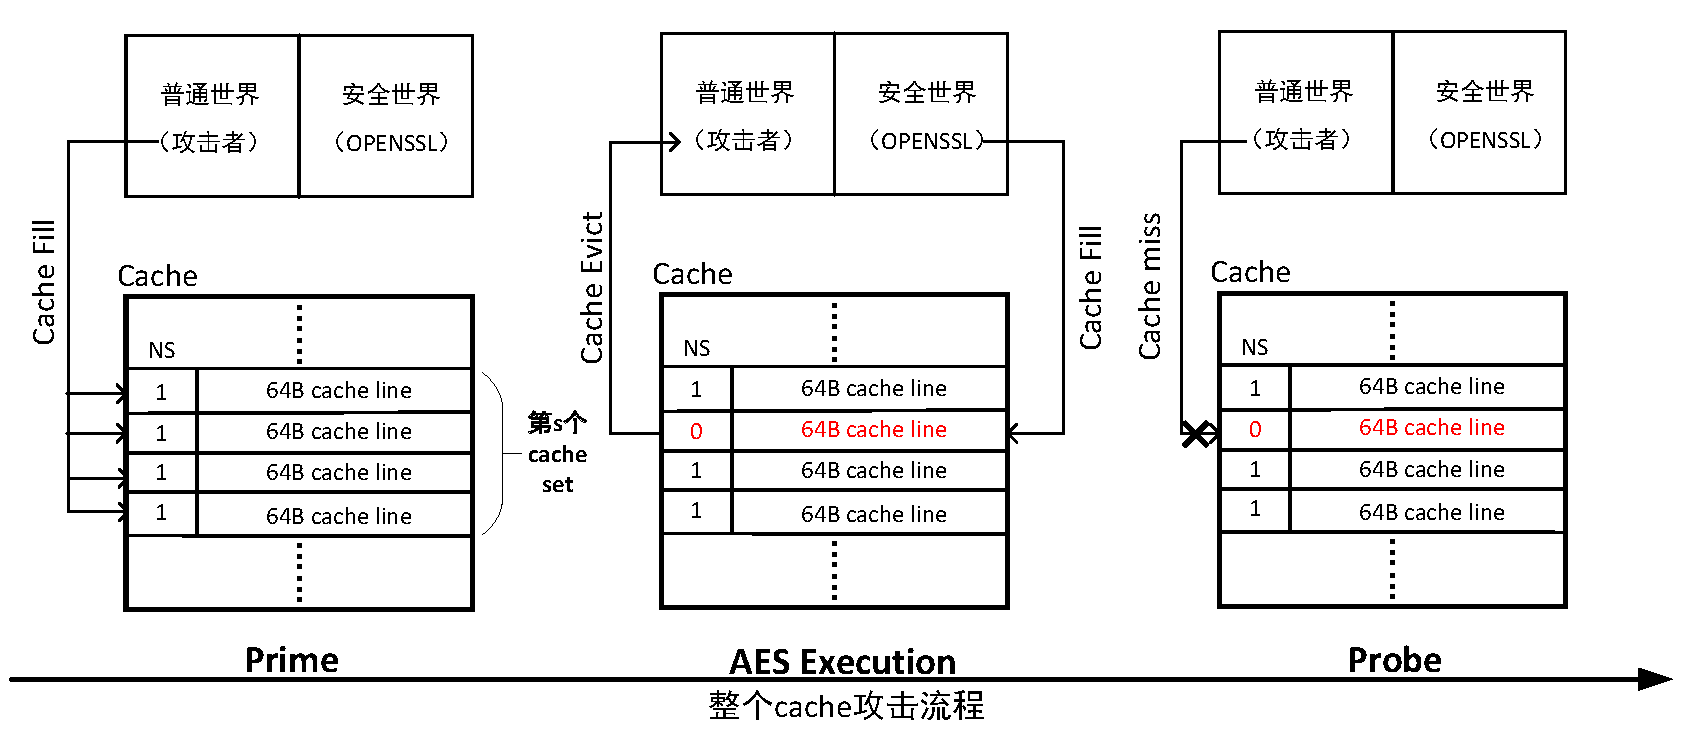
\includegraphics[width=0.95\textwidth]{005.png}
	\caption{对Te表的prime+probe缓存攻击}
	\label{005}
\end{figure}

Cortex-A53的每个缓存行有64字节,Te表的每一项为一个int类型数据,即4字节,因此每条高速缓存行拥有16个Te表项。一个Te表有256项,所以一个Te表所占用的大小为1KB,所占用的地址空间对应着16个缓存组,四个Te表的地址空间刚好占用了64个L1D缓存组。也就是说,给定一个缓存组的组号,可以唯一的对应到某个Te表的连续16个字节。在执行缓存攻击,当受害者执行AES的过程中,攻击者之前占据的某个缓存行会被驱逐,攻击者再进行检测时就会发现,该缓存行中16个可能的item中有一个被用于加密过程,因此,一次prime+probe缓存攻击将会产生16个可能的候选密钥字节。

理想情况下,攻击者需要中断加密过程,只使用上一轮改变的缓存配置来推断一轮中使用的密钥。但是,由于安全世界收到TrustZone的保护,在其中执行的AES加密过程是无法中断的,也就是说,当一次加密中的10轮加密全部结束后,我们才能获取一些被驱逐的表项,并且无法知道这个表项是在第几轮加密中被使用到的。这种不确定性需要用大量的样本量进行观测来弥补。

下面对大样本量可以弥补密钥不确定性进行可行性分析。假设$T{e_i}$在十轮中一共使用了m次,一个缓存组可以存放连续的16个表项,假设AES是在CBC模式下使用的,那么算法的输入可以被看作随机数,则加密过程中没有访问$T{e_i}$的16个连续表项的概率是${\left( {1 - \frac{{16}}{{256}}} \right)^m}$,因为一轮加密中需要用到4次Te表,故10轮加密则需要用到40次表项,平均到每个表即可以看作使用了10次,故代入m=40,可以得到概率值约为8\%。也就是说,任意一个缓存组有92\%的概率在一次加密中被使用,有8\%不会被用到,一次探测64个缓存组时,就有$64*8\%  = 5.12$的缓存组会检测不到cache miss,这些缓存组的Te表项就可以被完全排除。因此,通过探测更多的样本,可以排除更多的不可能密钥,经过多轮迭代,最终有能力推断出密钥的值。

\section{Neve\&Seifert排除法}

Neve\&Seifert排除法\cite{neve2006advances}是用上面得到的四个Te表的访问信息来得到加密密钥的算法。假设用Prime+Probe方法得到了一次加密中对四个Te表对应的缓存组的访问信息${P_i}\left( {0 \le i < 64} \right)$,${P_i}$为false 表示第$i$和$i+64$个缓存组均没有被使用,由于噪音的原因,${P_i}$为true的情况不予考虑。设${c_i}\left( {0 \le i < 16} \right)$为这一次加密的16字节密文。

规定$Te_{i + 2}^{'}\left[  \cdot  \right] = \left( {T{e_{i + 2}}\left[  \cdot  \right] >  > \left( {24 - 8i} \right)} \right)\& 0x{\rm{ff}}$为$GF\left( {{2^8}} \right) \mapsto GF\left( {{2^8}} \right)$的映射,由式 (4-12),可以得到$r{k_i} = {c_i} \oplus Te_{i + 2}^{'}\left[  \cdot  \right]$。以要恢复第0个字节的密钥为例,第0字节的密钥对应$T{e_2}$表的查表操作,若得知在加密过程中未访问到$T{e_2}$表以$t$开始的 16 个表项,则:

\begin{equation}
	\forall a \in \left[ {t,t + 16} \right),r{k_0} \ne {c_0} \oplus Te_2^{'}\left[ a \right]
\end{equation}

根据上式可以排除$r{k_0}$最多16个字节的取值,每一次攻击都累积记录这些非密钥的取值,当16个字节均只排除到只剩一个密钥时,证明所有非密钥已被排除,剩下的那个元素就是对应字节的密钥。

实现中,$T{e_0}$的第0项到$T{e_3}$的最后一项连续占用了一个内存页的全部地址空间,由于每个连续的16个T表项存在被放进0$-$63缓存组和64$-$127缓存组两个可能性,并且这是普通世界无法通过pagemap获取的信息,所以需要开辟一个数组${\rm{probe[128]}}$来探测一共128个缓存组的驱逐情况,即若${\rm{probe[s]}}$和${\rm{probe[s+64]}}$均未被访问,可以唯一地确定一个表的连续16项为非密钥,具体是$T{e_{\left[ {s/16} \right]}}$的第$\left( {s\bmod 16} \right)*16$至$\left( {s\bmod 16} \right)*16 + 15$项。

可以推出最后一轮中第$i$个密文字节的计算对应着$T{e_{i + 2}}$的查表操作(下标中加法为 GF(4)上的运算),设最后一轮密钥的16个字节的可能取值的集合为${K_i} = \left\{ {0,1,...255} \right\}$,并且每次排除法之后${K_i}$的结果可以继承。也就是说,每轮执行加密的时候,已经确定不是密钥的结果可以完全排除,不会出现在下一轮加密探测的可能密钥集中。在实现中,可以记录每一个${K_i}$集合中元素的个数,若个数为1,则说明排除密钥后只剩下一个可能的密钥了,也就是对应的密钥字节已经被恢复了,那么再接下来的轮数中,对这个密钥字节就可以直接跳过排除法步骤,这么做的目的是在攻击后期显著提升算法效率。

下面是Neve\&Seifert排除法的简要步骤:

\begin{breakablealgorithm}
	\caption{Neve\&Seifert排除法}
	\begin{algorithmic}[1]
		\Require probe结果${P_s}(0 \le s < 128)$,密钥候选${K_i}\left( {0 \le i < 16} \right)$,加密密文${c_i}\left( {0 \le i < 16} \right)$
		\Ensure 当$\left| {{K_i}} \right| = 1\left( {0 \le i < 16}$时的${K_i}$
		\Function{Elimination}{$P,K,C$}
		\For{$s=0\to 127$}
		\Comment{对128个缓存组分别进行遍历}
			\If{${P_s} =  = false$}
			\Comment{未检测到cache miss}
				\State $i\gets \left\lfloor {s/16} \right\rfloor  + 2\bmod 4$
				\While{$i<16$} % While语句,需要和EndWhile对应
				\Comment{对每一位的密钥候选项进行排除}
					\For{$j=0\to 15$}
					\Comment{每个cache set有16个Te表项}
						\State $K_i\gets {K_i}\backslash \left\{ {{c_i} \oplus Te_{i + 2}^{'}\left[ {\left( {s\bmod 16} \right) \times 16 + j} \right]} \right\}$
					\EndFor
					\State $i\gets i+4$
				\EndWhile
			\EndIf
		\EndFor
		\State $flag\gets true$
		
		\For{$i=0\to 15$}
			\If{$\left| {{K_i} \ne 1} \right|$}
			\Comment{每个$K_i$只剩一个值时即顺利攻击出密钥}
				\State $flag\gets false$
			\EndIf
		\EndFor
		\State\Return{$flag,K$}
		\EndFunction
	\end{algorithmic}
\end{breakablealgorithm}





\chapter{攻击方案}

\section{分配内存和缓存驱逐}
为了获得关于受害者进程对于缓存的具体访问情况,攻击者必须准确地将特定的内存填充到特定的缓存区域,这样它就会引起与受害者进程的缓存争夺。受害者的AES加密程序中的T表用到了128中的64个缓存组,需要首先填满128个缓存组,对于一个缓存组中的4路,我们需要准备4个互不相同且有效的物理地址,且都对应着这个缓存组,并且从物理地址起始的连续64个字节都可读,就可以填满这个缓存组的4个缓存行。可以利用pvalloc开辟出8个4K页面,同时利用/proc/self/pagemap控制其中的4个页面映射到前64个缓存组,另外四个页面映射到后64个缓存组。设基地址为$bas{e_i}$,低12比特都为0,且从$bas{e_i}$开始的连续4096个字节都是可读的。设对应缓存组号为$s$的对应驱逐地址为$evic{t_{s,i}}\left( {0 \le i < 8,0 \le s < 64} \right)$,则可以根据如下式子设计prime算法:

\begin{equation}
	evic{t_{s,i}} = bas{e_i} + \left( {s <  < 6} \right)
\end{equation}

64个缓存组刚好对应一整个4KB的页面的地址空间,故所开辟的8个页刚好可以直接填充128个缓存组。构造了内存驱逐集后,需要把所构造的数据放入缓存中。由于ARM处理器的缓存替代算法为随机替换,所以无法直接提出一个完全接近的替换算法,本文中,若要填充缓存组$s$,则把$evic{t_{s,i}}$从$i = 0\to 7$正向遍历若干次,实验中设置为10次,重复的次数若过多,则可能会让攻击效率下降,若过少,可能无法导致缓存组的数据被完全填充导致遗漏。遍历后,需要检查数据是否都被填充至L1缓存中,故在每次prime后都设置一次prime\_check,对所有数据检查访问的时间是否超过一定阈值,若没超过,则可以认为所有数据都已经被加载入L1 cache中,prime步骤就可以顺利完成。一旦有数据超过阈值,则认为在替换过程将之踢出缓存了,故需要重新进行prime过程,直到所有数据访问时间均未超过阈值。检查访问时间需要用到周期计数寄存器,将在下一节介绍。

\section{周期计数器探测缓存}



在执行了受害者的AES加密操作后,攻击者需要在普通世界中观测缓存的具体配置改变情况。由于安全世界的执行,需要探测此时缓存状态的变化。更具体地说,攻击者需要确定在prime步骤中填充的缓存行是否还在缓存中。我们从最高级缓存L1缓存的争夺中提取侧信道信息。因此,需要一个高精度的定时器来区分L1高速缓存或低级别的内存加载到寄存器中的时间上的不同。在x86系统中,可以使用rdtsc指令来提供纳秒级别的时间计时,在Skylake攻击平台上,甚至存在 MEM\_LOAD\_RETIRED.L1D\_MISS的事件可以直接记录L1d 缓存发生的cache miss次数。但是,在ARM处理器中,没有这样的计时器,但ARMv7架构提供了一个性能监控单元PMU,它有一个周期计数寄存器(PMCCNTR)。我们利用该周期计数寄存器来测量将内存或缓存载入寄存器所需的时间,以区分缓存层次结构中不同级别的缓存命中。

首先,为了在userspace能够正常使用PMCCNTR, 需要构造一个内核模块,并使用sudo insmod enable.ko命令激活。然后,我们以所示代码进行一个如何使用PMCCNTR的举例。指令流水线是许多现代处理器中用来实现指令级并行的技术,它使处理器的吞吐量更高,但它可能影响内存加载指令时间的测量,所以在周期计数寄存器被读取之前,使用isb指令(指令屏障)来完成流水线上的所有指令。此外,dsb(数据同步屏障)指令用来在定时器测量之前完成前面所有的操作。然后用ldr指令将存储在r3的内存地址加载到r0。dmb(数据内存屏障指令),用来等待前面访问内存的指令完成后再执行后面的指令。然后再读取周期计数器。两个定时器读数之间的差值被存储到r0中。按照类似的操作,可以完成所有指定的内存数据的探测。


\begin{lstlisting}[language=assembly]
	dsb
	isb
	mrc p15, 0, r1, c9, c13, 0
	ldr r0, [r3]
	dmb
	mrc p15, 0, r2, c9, c13, 0
	sub r0, r2, r1
\end{lstlisting}

一旦时间被记录下来,就可以与提前测好的已知阈值进行比较,从而对内存访问的级别进行分类。不同级别的内存访问(L1、L2、DRAM)可以通过Cortex-A53的性能单元中的周期计数寄存器区分出来。经过实验,L1缓存上的缓存命中平均有90个CPU周期,而从L2缓存加载使用127个CPU周期,从内存加载数据则需要311个CPU周期。因此,周期计数寄存器使攻击者不仅能可靠地分辨出缓存缺失和缓存命中之间的区别,还能分辨出缓存命中的缓存级别。利用其中的时间差,在probe阶段,我们可以判断每加载一个64B的数据时,所耗费的CPU周期,如果没有超过90这个CPU周期阈值,我们就认为此时的数据仍是从L1D cache中加载的,也就是说受害者进程在执行AES加密时,并没有用到这个地址对应的缓存组中的数据。因为我们提前可以知道这个缓存组中的16个T表项的具体内容,结合获得的密文,对于每个字节,我们就可以直接排除对应的16个可能的密钥值。


\section{普通世界与安全世界交互设计}

前文中提到,普通世界提供AES加密的16字节明文,唤醒安全世界的加密程序执行,并能够获得加密之后的16字节密文,本节将阐述实验中如何设计两个世界的程序交互过程。

普通世界和安全世界的程序可以看作CA(Client Application,运行在普通世界)和TA(Trust Application,运行在安全世界)两端的交互或者通话过程。典型的CA有支付应用、指纹对比等,利用特定接口调用可信执行环境中的服务,其中的具体过程对于CA端是透明且无法得到的。TA是可信执行环境中完成特定功能的应用,这些应用通常具有较高安全性,执行特定服务后将计算结果返回给调用自己的CA。

CA在用户层面调用CA接口以后就会产生系统调用(system call)操作,系统调用会使Linux进入内核状态(kernel space),此时操作系统将处于内核区域,然后通过传入的参数,当SMC中断处理函数实现了将cortex的状态转换到安全世界和对相关参数的拷贝之后,安全世界中的操作系统将进行下一步的处理。操作系统首先会得到传过来的数据信息以及想要的TA的UUID,并加载对应的TA image。然后,安全世界中的操作系统会转换到TEE 用户态,并将CA传递过来的其他参数传给TA。当TA获取到参数之后,首先解析出参数中的commond ID值,根据具体的command ID值来做对应的操作,例如指纹对比、加解密操作。等操作执行完成后,会根据之前的过程,依次回退,最后的结果将会传递给CA端,CA端将获取可信服务的结果。整体流程可以参考图\ref{007}。

\begin{figure}[H]
	\centering
	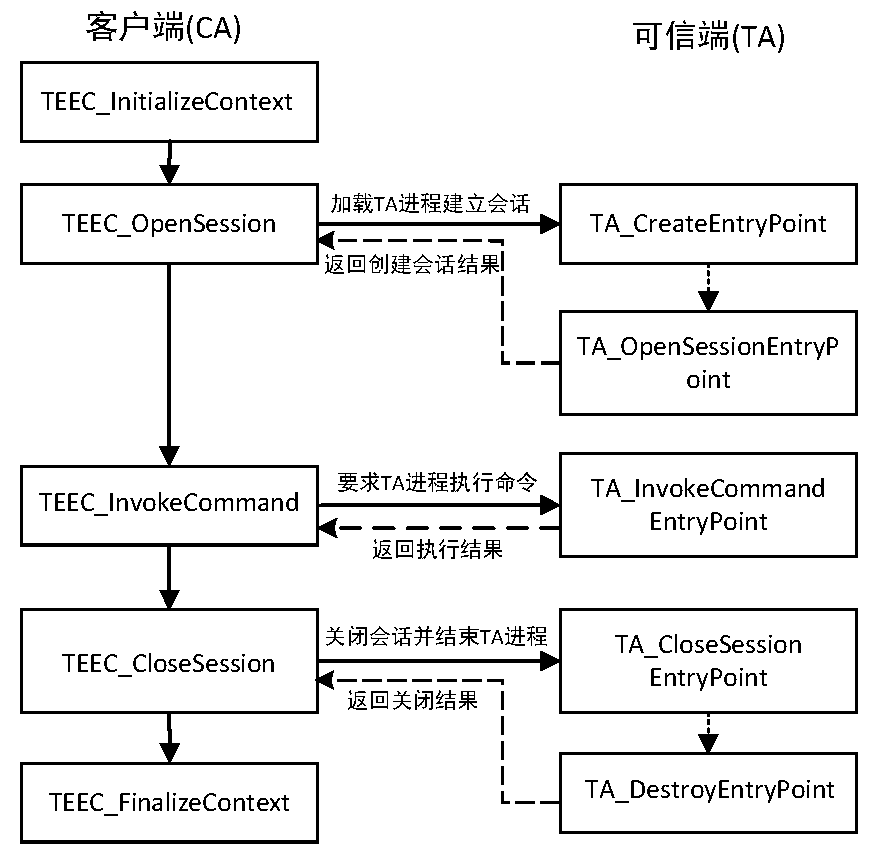
\includegraphics[width=0.7\textwidth]{007.png}
	\caption{TA与CA交互设计}
	\label{007}
\end{figure}

CA就是在REE中用来控制TA的应用程序,典型的CA程序流程遵循GP客户端API。主要包含五个与TA中对应的api来控制CA-TA连接与指令操作。一次完整的CA调用过程需要分别实现以下五个接口操作:

\begin{itemize}
	\item TEEC\_InitializeContext: 通过初始化TEE上下文变量(context),以建立与TEE之间的通话通道
	\item TEEC\_OpenSession: 建立CA与TA之间的会话窗口
	\item TEEC\_InvokeCommand: 向TA发送command请求来执行具体的操作
	\item TEEC\_CloseSession: 关闭CA与TA之间的对话窗口
	\item TEEC\_FinalizeContext:清空会话通道,清除context变量
\end{itemize}

结合本文实验的加密操作,具体来说,完成一次完整的CA请求时,程序需要执行的操作分别是:首先调用TEEC\_InitializeContext函数,获取ctx变量并存放到TEE\_Context类型的变量中。然后调用TEEC\_OpenSession函数,创建一个CA与特定TA之间进行通信的通道。然后需要初始化TEEC\_Operation类型的变量,由于CA端需要提供明文,故该变量第一个参数类型需设置为TEEC\_MEMREF\_TEMP\_INPUT,并且在变量中存放明文内容和字节数。使用规定的command ID作为参数,调用TEEC\_InvokeCommand函数来真正发起对应的加密请求。之后的具体加密实现将由OP-TEE和TA进行处理,并将得到的密文返回给CA端。调用成功之后需要注销会话变量sess,并且释放掉ctx,这两个操作一次通过调用TEEC\_CloseSession函数和TEEC\_FinalizeContext函数来实现。TA端的实现同样使用五个与上述对应的API来控制CA-TA连结与指令操作:

\begin{itemize}
	\item TA\_CreateEntryPoint:建立进入点,让TA可以被呼叫
	\item TA\_OpenSessionEntryPoint:建立CA呼叫TA的通道session
	\item TA\_InvokeCommandEntryPoint:接收CA传送的指令,执行对应函数
	\item TA\_CloseSessionEntryPoint:关闭CA-TA的通道
	\item TA\_DestroyEntryPoint:移除进入点,结束TA的功能
\end{itemize}

在本文设置的实验中,完成一次加密操作的TA端,程序需要定义以下的内容:TA\_CreateEntryPoint和TA\_OpenSessionEntryPoint分别对应了CA端的前两个api,完成这两步后,TA端就已经和CA端进行了加密操作的连接。TA\_InvokeCommand EntryPoint()函数则为CA端发起加密请求时对应的操作接口,因为本文中的TA端设置了两个加密服务,分别是初始化密钥以及加密操作,TA根据传入的值,决定跳转到TEE\_Result aes\_init()或TEE\_Result aes\_encrypt()函数进行处理。初始化密钥函数中随机生成一个16字节密钥,利用密钥扩展操作初始化加密密钥。加密函数接收传过来的明文以及对应字节数,在函数内部对明文进行openssl的加密调用,并且生成16字节密文,同样放入参数中传回给CA端。TA\_CloseSession EntryPoint和TA\_DestroyEntryPoint同样对应了CA端的后两个api,当被调用后,整个连接将被终端,剩下的操作将交给普通世界中的程序进行缓存侧信道攻击。

\section{攻击算法流程}

为了模拟真实的攻击环境,AES加密的密钥由tee内TA产生,外部攻击者无法直接获取,外部攻击者CA可以通过TEEC\_Operation类型的参数来传递加密的明文和获取加密的密文。为了进一步减少噪音,本攻击设置了 Linux 进程调度优先级,将攻击者线程的优先级调至最高,以保证攻击者在整个攻击阶段的程序不会被其他线程干扰,此过程需要root权限。


具体的普通世界与安全世界的交互设计见图\ref{008}。在攻击前,攻击者指定一个特定的16字节明文,获取它的TrustZone加密结果,存储起来。然后攻击者正式开始攻击过程,在每一次的prime+probe过程中,都随机生成一个明文,发送给受害者进行加密,并通过密文及缓存信息结合排除法进行密钥的筛选。在攻击者通过排除法把所有的密钥取值候选值都只剩余1个时,攻击者通过最后一轮的密钥,计算出最初的加密密钥,用这个密钥去解密前面存储的密文,若与指定的明文相同,则说明攻击密钥恢复成功。

\begin{figure}[H]
	\centering
	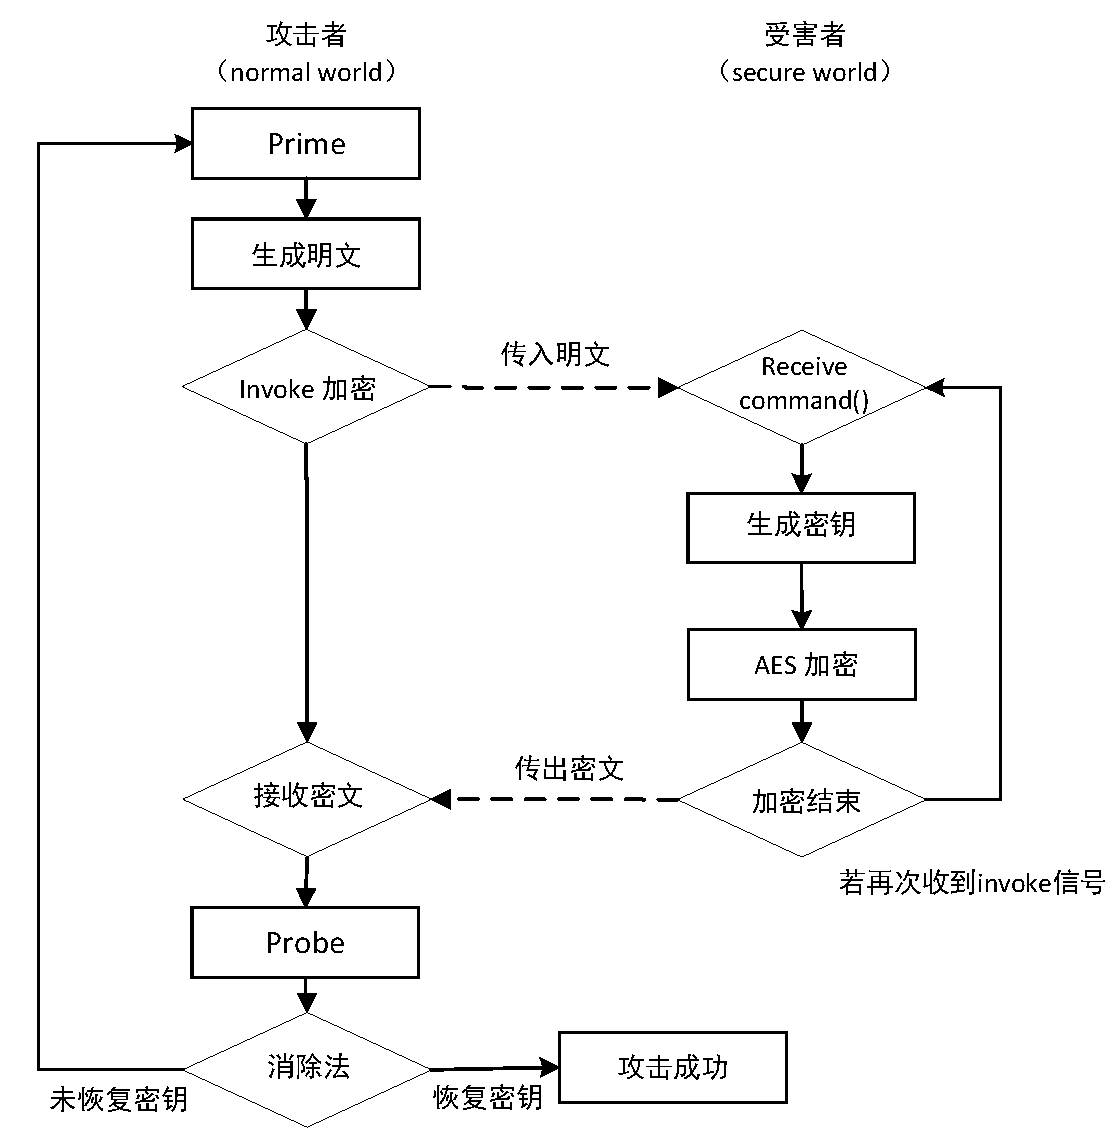
\includegraphics[width=0.8\textwidth]{008.png}
	\caption{攻击算法流程}
	\label{008}
\end{figure}




\chapter{实验与分析}
\section{攻击结果与性能分析}
本小节介绍实验中的攻击结果以及相关性能分析。实现攻击的硬件平台为Cortex-A53处理器armv7l架构,有四个物理核。攻击环境是Linux Raspbian GNU/Linux 10 (buster),内核版本为4.14.98-v7,所有ta端编译得到的.ta文件均放在/lib/optee\_armtz文件夹中。

在teecache目录下输入sudo LD\_LIBRARY=\$(HOME)/teeaes\_aes ./spy,并且循环1000次攻击,即可得到以下攻击结果。可以看到受害者提前生成一个密钥,这个密钥攻击者是不可知的,只是为了可视化展示输入在屏幕上。攻击者发送明文并且收到加密密文。利用上一章介绍的算法流程,对缓存进行prime+probe攻击,最终恢复了最后一轮密钥,并由aes128\_key\_schedule\_inv\_round函数得到了最初的密钥,利用这个密钥对收到的密文进行解密,得到的明文与最初发送的明文一致,故攻击成功。


\begin{figure}[H]
	\centering
	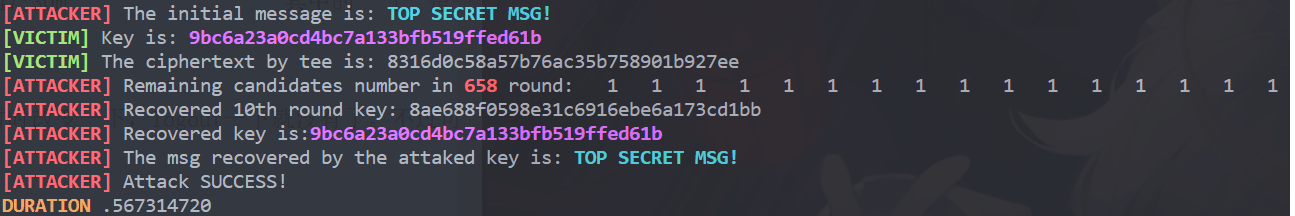
\includegraphics[width=0.9\textwidth]{009.png}
	\caption{攻击结果}
	\label{009}
\end{figure}



除了上述的排除法,还可以利用投票法计算猜测熵(Guessing Entropy, GE),以此估计该侧信道攻击的可靠性。猜测熵在侧信道攻击中,是对攻击者猜测系统效果的常用评估手段。在本文的实验中,在probe步骤之后,得到了没有发生cache miss的缓存组对应的Te表项,对这些表项的vote值进行投票累加,同时对整个prime+probe过程规定固定次数。当遍历完规定次数后,观察每个字节的256个vote值,其中投票次数最少的为该字节最有可能的密钥。因为每种攻击算法最后不一定能攻击出正确的密钥,故可以将正确的密钥对应的投票数在所有投票数中进行排序,若最后得到投票数最少,记猜测熵为1,表明攻击效果较好,能成功攻击出密钥,猜测熵越大,可以看作攻击效果越差,即${\rm{GE}}\left( {byt{e_i}} \right) = r{k_i}$。


\begin{figure}[H]
	\centering
	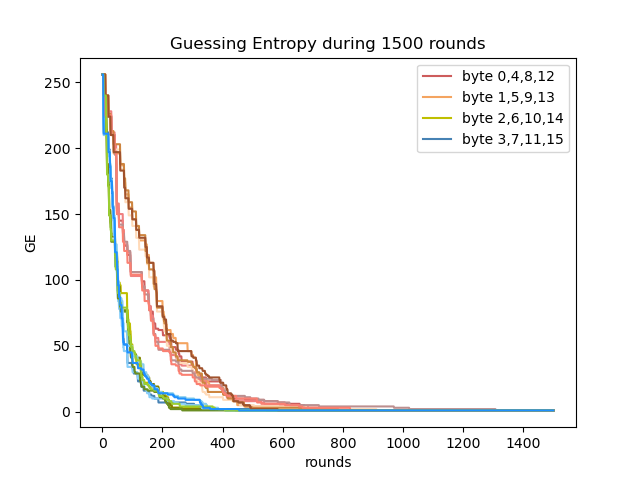
\includegraphics[width=0.75\textwidth]{015.png}
	\caption{猜测熵随轮数变化情况}
	\label{015}
\end{figure}


图\ref{015}为任意50次攻击的平均猜测熵下降图,图中将同色系作为不同位置字节的标识。可以看到,整体的下降趋势和图\ref{010}类似,但反应的信息更详细。首先,每个字节在规定的1500次遍历后,GE均下降到1,证实了攻击的有效性。每个色系的字节在加密过程中的位移或占用的Te表都是相等的,所以攻击速度也相互接近。蓝色和绿色系的字节在400轮左右猜测熵已经降为1,红色系对应的字节虽然一开始下降较快,但是直到1000轮左右才完全猜测出密钥,证明${P_i}\left( {0 \le i \le 3} \right)$中的第一个字节是攻击的关键,决定了攻击的整体速度,具体原因有可能是调用tee过程中的内存所对应的缓存组正好与之相同,导致攻击者在前期一直无法探测出。


\section{cache攻击应对方法}

自从近二十年前第一个基于缓存的时间侧信道攻击被提出,学术界已经做了很多研究来推进对缓存信息侧信道的攻击和防御。与以前的工作类似,本文研究的最终目标是进一步了解TrustZone安全世界中的侧信道信息泄露,并优化未来的设计。对侧信道攻击的防御通常遵循两个方向。第一个方向试图在加密操作本身的实现上下功夫,而第二个方向则侧重于加固加密操作所运行的系统,以消除在时间上的侧信道信息。这部分主要介绍一些可能的解决缓存侧信道攻击的方法。

在改进加密算法的方法中,最直接的方法是关注加密算法本身。OpenSSL采用了一种缓解措施来预装AES的T表,这样,假设加密算法的执行不能被打断,对该表的访问就不能再被攻击者发现,也就是说,攻击者连T表的逻辑地址等基本信息都无法获得,更不能得到对应的缓存组信息了。还有一些防御性的措施,例如将软件控制流随机化\cite{crane2015thwarting},这样执行路径和缓存组之间就没有固定的关系,一旦没有这种映射信息,攻击者就不可能从高速缓存配置中推断出重要数据,也就不能汇总统计数据来推断密钥。

在加固加密操作所运行的系统这个方向上,我们需要先着重了解破解高速缓存时间侧信道攻击的两个要求。首先,攻击者必须能够用内存填满缓存,以造成与受害者进程的资源争夺,因此可以试着消除这种资源争夺。由于内存分配是由内核指定的,一个操作系统级攻击者,在完全控制所有普通世界内存的情况下,可以成功攻击秘密值。那么,为了组织这种缓存争夺,我们可以规定程序对缓存的使用,最简单的就是关闭缓存,完全关闭缓存肯定会影响程序的运行效率,但如果操作系统可以提供一些特殊的操作,允许程序自行决定是否可以启用缓存,受害者程序可以选择在执行涉及到秘密数据的时候关闭缓存,这样对整体的运行效率不会产生太大的影响。类似原理的操作还可以是,不关闭缓存的使用,但是给安全世界内的程序划分特定的缓存隔离区域,也就是跟内存一样的分隔机制,这些缓存内容是不能被其他程序或操作系统读写的,并且在该程序执行完成后会自动销毁并回收。

创建高速缓存侧信道的第二个要求是能够检测缓存状态的变化。因此,攻击者需要一个高精度的定时器来区分来自内存系统不同层次的内存访问。如果我们能限制访问内核性能事件接口的权限,有可能可以防止非内核权限的应用对安全世界侧信道信息的访问。



\chapter{总结与展望}
\section{方案总结}
本文先介绍了ARM TrustZone可信执行环境的运行原理,然后分析了4种现代常用的缓存攻击方法。由于TrustZone的内存分离机制,只有prime+probe攻击是无法抵抗的。我们实践了基于时间的缓存侧信道攻击,能够从TrustZone的安全世界中提取密钥,即开发了一个攻击模式,其中攻击者拥有操作系统最高权限,通过触发在安全世界里执行的AES加密,最终证实可以在0.75秒左右进行大约801.07轮观察的AES加密,并且成功从安全世界中提取完整的16位AES加密密钥。由于我们的攻击依赖于启用TrustZone的缓存架构的基本设计,因此理论上它对各种版本的ARM处理器均有效。最后,本文提出了可能的缓存攻击预防策略。


\section{未来工作}
本文使用AES作为从信任区的安全世界中提取重要或敏感信息(如秘密密钥)的能力的示范。然而,它的适用性绝不仅限于AES。在AES中跟踪T表访问的方法也可以应用于其他基于表的加密实现\cite{irazoqui2015s,liu2015last}。同时,当安全世界内的程序使用内核地址空间布局随机化(KASLR)\cite{hund2013practical}时,同样可以使用类似的缓存侧信道手段进行攻击。

从其他平台的应用来考虑,尽本文的原理并不局限于单核处理器,因为我们目前的实现使用最高级的L1数据高速缓存来减少噪音,但还需要一些进一步的研究来扩展这种方法在多核处理器上的机制。在许多现代多核处理器中,每个单独的处理器内核都有自己的专用L1高速缓存。为了继续利用L1上的缓存争夺作为侧信道信息的来源,攻击需要被安排和受害者处在同一个处理器核心上运行,这通常很难实现。

另一方面,最后一级缓存通常由所有内核共享,以前的一些工作主要是利用最后一级缓存作为侧信道信息的来源\cite{irazoqui2015s,liu2015last,ristenpart2009hey}。当把这种方法扩展到多核处理器(如ARMCortex-A9)时,攻击需要使用最后一级共享缓存来应用prime+probe技术。然而,在一些ARM处理器上,如CortexA-9,缓存控制器拥有inclusive的特点,以确保存在高层缓存中的任何缓存行也存在于低层缓存中,那么,对最后一级缓存的探究将可能受到其它核的高级缓存的操作影响,这种情况下,低级缓存中可能存在额外的噪音,将给攻击提升一定的难度。因此,对其它加密方法的应用、对多核处理器的应用以及对具有inclusive特性的最后一级缓存的应用,都可以成为将来prime+probe缓存侧信道攻击在ARM架构处理器上的研究对象。
